\Chapter{ADAPTIVE SAFE SCREENING METHOD FOR ELASTIC NET WITH SPARSE RULE}
\label{METHOD3}

\section{Introduction}

Consider the linear regression setting with $n$ samples and $p$ features, and let $\boldsymbol y$ denote the vector of $n$ responses and $X=[\boldsymbol x_1,...,\boldsymbol x_p]$ denote the $n\times p$ matrix of features. The elastic net \citep{zou2005regularization} is defined by the optimization problem 
\begin{equation}
    \label{eq:enet0}
    \underset{\beta\in \mathbb{R}^p}{\mathrm{min}}\frac{1}{2}\norm{\boldsymbol y-X\boldsymbol\beta}_2^2+n\lambda_1\norm{\boldsymbol\beta}_1+\frac{n}{2}\lambda_2\norm{\boldsymbol\beta}_2^2,
\end{equation}
where $\lambda_1,\lambda_2> 0$ are tuning parameters that control the sizes of the $L_1$ and $L_2$ penalties and $\boldsymbol\beta\in\mathbb{R}^p$ is the coefficient vector for the $p$ features. In practice, the elastic net is typically reparameterized as
\begin{equation}
    \label{eq:enet}
    \underset{\beta\in \mathbb{R}^p}{\mathrm{min}}\frac{1}{2}\norm{\boldsymbol y-X\boldsymbol\beta}_2^2+n\alpha\lambda\norm{\boldsymbol\beta}_1+\frac{n(1-\alpha)}{2}\lambda\norm{\boldsymbol\beta}_2^2,
\end{equation}
where the tuning parameter $\lambda>0$ controls the overall size of penalty and $\alpha\in(0,1)$ controls the balance between $L_1$ and $L_2$ penalties. This parametrization allows us to tune only the overall size $\lambda$ while keeping $\alpha$ fixed, instead of tuning $\lambda_1$ and $\lambda_2$ at the same time. Since this parameterization makes the tuning parameters both more interpretatble and easier to select, it is usually more preferable in practice. For example, it is the parameterization that appears in the most widely used in the R package \textbf{glmnet}, the most widely used software for fitting elastic net models. For the rest of the paper, we focus only on the reparametrized problem \eqref{eq:enet} and treat $\lambda$ as the only tuning parameter.

The elastic net is a regularization method very similar to the lasso \citep{tibshirani1996regression}; the only difference is the addition of an extra $L_2$ penalty. Like the lasso, elastic net solutions are sparse and enjoy the benefits of shrinkage. The additional $L_2$ penalty, however, offers several appealing advantages over the lasso method. First, the objective function in elastic net problem \eqref{eq:enet} is strictly convex so there is always a unique solution. The lasso solutions, on the other hand, may not be unique; this most commonly occurs in high dimensional problems and when the regularization parameter is small. Second, when a group of important features is highly correlated, the elastic net tends to select the entire group, whereas the lasso tends to select only one of them.

The elastic net and lasso methods have had great success in high dimensional data analysis, where the number of features $p$, and possibly also the sample size $n$, are very large. Efficient algorithms to solve them are important because the dimensionality introduces considerable costs in terms of time and memory. One of the most promising techniques, and one that can be used in combination with any other algorithm, is \quotes{screening}, which takes advantages of sparsity: if we knew which coefficients would be 0 in the solution before solving the problem, we could \quotes{eliminate} those features from the problem. Any algorithm could then be applied to the reduced problem and would be much faster, but the solution would be exactly the same as the solution to the origin problem. In practice, we can never know all the sparse features, but can attempt to identify and eliminate as many features as possible without making any incorrect eliminations. A typical practice is to solve penalized regression problems sequentially along a path of regularization parameter values $\lambda_0,\lambda_1,...,\lambda_L$, then select the best value. In this case, when solving the problem at $\lambda_l$, solutions at previous values $\lambda_0,...,\lambda_{l-1}$ are already known. Because solution paths are continuous, there are constraints on how far away one solution can be from the previous one, and therefore previous solutions can be used to construct powerful screening rules to potentially eliminate a large number of features. There have been many studies of screening methods for the lasso problem \citep{ghaoui2010safe,Tibshirani2012,wang2013lasso,fercoq2015,Zeng2021} and the work in this area has let to significant improvements in the speed of popular lasso algorithms.

Screening methods for the elastic net, however, are still very limited. If we consider the naive form \eqref{eq:enet0} and treat $\lambda_2$ as fixed, then the $L_2$ penalty can be incorporated into the loss, making the problem equivalent to the lasso problem and allowing the use of lasso screening methods \citep{xu2019}. However, this is not relevant in practice as it is form \eqref{eq:enet} that is actually used in real data analysis. Zeng et al. \citep{Zeng2021} proposed the BEDPP screening rule for elastic net, but it cannot utilize previous solutions and as a result rapidly loses power along the solution path. There are, however, unsafe screening rules such as the strong rule \citep{Tibshirani2012} that can be applied to the elastic net. Such rules, however, require post-convergence checks to make sure no features were mistakenly eliminated. Strong rules nevertheless provide significant speedups in a large class of problems including the lasso and elastic net, and have been widely used, for example, in \textbf{glmnet}. However, recently, the adaptive screening framework proposed in Chapter \ref{METHOD1}, which adaptively reuses previous solutions as a reference when applying safe screening rules, has been shown to outperform other screening methods, including strong rule screening, by a large margin for solving the lasso problem. This framework has not yet been applied to the elastic net, however, as no safe screening rule that can utilize previous solutions has been developed.

In this paper, we propose a powerful, adaptive safe screening method for the elastic net problem that efficiently utilizes previous solutions as references. In section 2 we derive the Sequential Projecting And Reshaping Safe Elimination (SPARSE) rule and incorporate it into the adaptive screening framework to form an adaptive screening method. In section 3, we carry out experiments on both synthetic and real data sets to compare our method with strong rules, the other state-of-the-art screening method. In section 4, we discuss the results and some some additional remarks.

\section{Screening Method}
\subsection{Problem Formulation}
\label{sec:formulation}

A dual formulation of problem \eqref{eq:enet} can be given by (see Appendix \ref{sec:duale} for details):
\begin{gather}
        \label{eq:dualtheta}
        \underset{\boldsymbol\theta\in \mathbb{R}^{ n},\boldsymbol\gamma\in\mathbb{R}^p}{\mathrm{max}}g_\lambda(\boldsymbol\theta,\boldsymbol\gamma)\equiv\frac{1}{2}\norm{\boldsymbol y}_2^2-\frac{\lambda^2}{2}\left\Vert\boldsymbol\theta-\frac{\boldsymbol y}{\lambda}\right\Vert_2^2-\frac{\lambda^2}{2}\norm{\boldsymbol\gamma}_2^2\\
        \begin{aligned}s.t.\quad (\boldsymbol\theta,\boldsymbol\gamma)\in \mathcal{F}_\lambda\equiv\{(\boldsymbol\theta,\boldsymbol\gamma):\quad
            &\norm{X^T\boldsymbol\theta-\sqrt{n(1-\alpha)\lambda}\boldsymbol\gamma}_\infty\leq n\alpha\}\nonumber,
        \end{aligned}
\end{gather}
where $\boldsymbol\theta\in \mathbb{R}^{n}$ and $\boldsymbol\gamma\in\mathbb{R}^p$ are the dual variables. We will use $\boldsymbol\mu\in \mathbb{R}^{n+p}$ to denote the combined vector $(\boldsymbol \theta,\boldsymbol\gamma)$. The dual problem consists of minimizing the convex function $g_\lambda(\boldsymbol\mu)$ within a convex feasible set $\mathcal{F}_\lambda$. Geometrically, the problem is equivalent to projecting $(\frac{\boldsymbol y}{\lambda},0)$ onto $\mathcal{F}_\lambda$. Letting $\boldsymbol\beta_\lambda$ denote the solution to the primal problem at penalty parameter value $\lambda$ and $\boldsymbol\mu_{\lambda}=(\boldsymbol\theta_{\lambda},\boldsymbol\gamma_\lambda)$ denote the corresponding dual solution, the primal solution and dual solutions are connected by
\begin{equation}
    \label{eq:dualprimal}
    \boldsymbol\theta_\lambda=\frac{\boldsymbol y-X\boldsymbol\beta_\lambda}{\lambda},\quad \boldsymbol\gamma_\lambda=\sqrt{\frac{n(1-\alpha)}{\lambda}}\boldsymbol\beta_\lambda.
\end{equation}
Furthermore, the KKT conditions for the primal problem~\eqref{eq:enet} can be expressed as:
\begin{gather}
    \label{eq:kkte}
    \begin{aligned}&[\boldsymbol\beta_\lambda]_{j}=0\implies|\boldsymbol x_j^T\boldsymbol\theta_\lambda|\leq n\alpha\\
    & [\boldsymbol\beta_\lambda]_{j}\neq0\implies  \boldsymbol x_j^T\boldsymbol\theta_\lambda-n(1-\alpha)[\boldsymbol\beta_\lambda]_{j}=n\alpha\,\textrm{sign}([\boldsymbol\beta_\lambda]_{j}).
    \end{aligned}
\end{gather}
for any $j$. Combining \eqref{eq:dualprimal} and \eqref{eq:kkte} we have a trivial closed form solution for the problem at large $\lambda$ values:
\begin{gather}
    \label{eq:lammax}
    \begin{aligned}
        \boldsymbol\beta_\lambda=0\iff \lambda \geq \lambda_{\max}\equiv \max_j \frac{|\boldsymbol x_j^T\boldsymbol y|}{n\alpha}
    \end{aligned}
\end{gather}
Thus, when solving the problems on a grid of $L+1$ decreasing $\lambda$ values: $\lambda_0>\lambda_1>...>\lambda_L>0$, it makes more sense to choose $\lambda_0=\lambda_{\max}$ to take advantage of the known solution. If an algorithm solves the problems sequentially in decreasing order of $\lambda$, then the solution at $\lambda_{l'}$ will be known before solving the problem at $\lambda_l$ if $l'<l$. In the rest of this section, we will derive a screening method for this pathwise approach. Also, without loss of generality, we will derive the screening method for the problem at $\lambda_1$ assuming the solution at $\lambda_0$ is known and can be used as a reference for screening. We refer to this pair as the \quotes{target} ($\lambda_1)$ and the \quotes{reference} ($\lambda_0$). The same method can be applied to any pair of $\lambda_{l}$ and $\lambda_{l'}$. For simplicity, we will use $\boldsymbol\beta_l,\boldsymbol\mu_l,\boldsymbol\theta_l,\boldsymbol\gamma_l$ to denote the solution at any $\lambda_l$.

Note that from the KKT conditions \eqref{eq:kkte}, if
\begin{equation}
    \label{eq:disc_cond}
    |\boldsymbol x_j^T\boldsymbol\theta_{1}|<n\alpha,
\end{equation}
we can safely conclude $\boldsymbol\beta_{1,j}=0$ and the corresponding $\boldsymbol x_j$ can be eliminated for the optimization at $\lambda_1$. Although the left hand side of \eqref{eq:disc_cond} is unknown until the solution is obtained at the target $\lambda_1$, we can use the solution at the reference $\lambda_{0}$ to derive some upper bound for the left hand side: $T_j(\lambda_{1},\lambda_{0}|\boldsymbol\mu_0)\geq |\boldsymbol x_j^T\boldsymbol\theta_1|$ and then if $T_j(\lambda_{1},\lambda_{0}|\boldsymbol\mu_0)<n\alpha$ we can also safely conclude $\boldsymbol\beta_{1,j}=0$. The goal is to find as small a bound $T_j(\lambda_{1},\lambda_{0}|\boldsymbol\mu_0)$ as possible, as this will maximize the number of features we are able to eliminate. An important technical challenge posed by the elastic net problem is that as $\lambda$ changes, both the dual function $g_\lambda$ and the feasible set $\mathcal{F}_\lambda$ change. In comparison, for the lasso the dual function changes with $\lambda$ but the feasible set remains constant.

To simplify the construction of the upper bound, we consider the intermediate dual problem:
\begin{gather}
        \label{eq:dualmi}
        \boldsymbol\mu_{1|0}=(\boldsymbol\theta_{1|0},\boldsymbol\gamma_{1|0})\equiv\underset{\boldsymbol\mu\in \mathbb{R}^{ n+p}}{\mathrm{arg\,max}}\,g_{\lambda_0}(\boldsymbol\mu)\\
        \begin{aligned}s.t.\quad \boldsymbol\mu\in \mathcal{F}_{\lambda_1}\nonumber.
        \end{aligned}
\end{gather}
Compared to the original dual problem \eqref{eq:dualtheta} at the reference $\lambda_0$, the intermediate problem \eqref{eq:dualmi} optimizes the same dual function on a reshaped feasible set. On the other hand, compared to the intermediate problem, the original dual problem at the target $\lambda_1$ optimizes a slightly different dual function on the same feasible set, or geometrically, projects a slightly different point on the same feasible set. The main idea of the proposed SPARSE rule is that it is difficult to establish bounds by directly considering the target-reference pair of problems because the dual function and feasible set are both changing, but by considering the intermediate-reference and intermediate-target pairs, the problem becomes two tractable reshaping and projection problems. Specifically, we can find a region $\mathcal{A}^1(\lambda_1,\lambda_0|\boldsymbol\mu_0)$ based on the reference solution $\boldsymbol\mu_0$, that contains the intermediate solution ($\boldsymbol\mu_{1|0}\in \mathcal{A}^1(\lambda_1,\lambda_0|\boldsymbol\mu_0)$) and subsequently find a region $\mathcal{A}^2(\lambda_1,\lambda_0|\boldsymbol\mu_{1|0})$ based on the intermediate solution $\boldsymbol\mu_{1|0}$, that contains the target solution  ($\boldsymbol\mu_1\in \mathcal{A}^2(\lambda_1,\lambda_0|\boldsymbol\mu_{1|0})$). Finally, if we find an upper bound for the double maximization problem over the two regions,
\begin{equation}
    \label{eq:boundbound}
    T_j(\lambda_{1},\lambda_{0}|\boldsymbol\mu_0)\geq \underset{\boldsymbol\mu'\in\mathcal{A}^1(\lambda_1,\lambda_0|\boldsymbol\mu_0)}{\mathrm{max}}\,\underset{\boldsymbol\mu\in\mathcal{A}^2(\lambda_1,\lambda_0|\boldsymbol\mu')}{\mathrm{max}}|\boldsymbol x_j^T\boldsymbol\theta|,
\end{equation}
then it automatically satisfies $T_j(\lambda_{1},\lambda_{0}|\boldsymbol\mu_0)\geq |\boldsymbol x_j^T\boldsymbol\theta_1|$ and can be safely used for screening. Note that one could also construct an intermediate problem by first changing the objective function while the feasible set remains the same; this alternative method is briefly discussed in Appendix \ref{sec:alternative-method}.

Let $c$ and $d$ denote the following scalar quantities, which appear in several expressions throughout this section:
\begin{equation}
    c\equiv\frac{\lambda_0-\lambda_1}{\lambda_0\lambda_1},\quad d\equiv \frac{\sqrt{\frac{\lambda_1}{\lambda_0}}+\sqrt{\frac{\lambda_0}{\lambda_1}}}{2}.
\end{equation}

In the special case when $\lambda_0=\lambda_{\max}$ as defined in \eqref{eq:lammax}, a form of the bound $T_j(\lambda_{1},\lambda_{0}|\boldsymbol\mu_0)$ has previously been derived \citep{Zeng2021} and which we restate below. Thus, in rest of this section, we focus on the case when $\lambda_0<\lambda_{\max}$. Together, these two cases cover the entire solution path.

\begin{theorem}
    \label{thm:0.1}
    For any $\lambda_1\in(0,\lambda_{0})$, let $\boldsymbol x_*\equiv\underset{\boldsymbol x_j}{argmax}|\boldsymbol x_j^T\boldsymbol y|$, if $\lambda_0=\lambda_{\max}$, then
    \begin{gather}
        \begin{aligned}
            T_j(\lambda_{1},\lambda_{0}|\boldsymbol\mu_0)&=\left|\frac{\lambda_{0}+\lambda_1}{2\lambda_{0}\lambda_1}\boldsymbol x_j^T\boldsymbol y-\frac{n\alpha c\lambda_{0}}{2(\norm{\boldsymbol x_*}_2^2+n(1-\alpha)\lambda_1)}\textit{sign}(\boldsymbol x_j^T\boldsymbol y) \boldsymbol x_j^T\boldsymbol x_*\right|+\\
            &\frac{c}{2}\sqrt{\left(\norm{\boldsymbol x_j}_2^2+n(1-\alpha)\lambda_1\right)\left(\norm{\boldsymbol y}_2^2-\frac{n^2\alpha^2\lambda_{0}^2}{\norm{\boldsymbol x_*}_2^2+n(1-\alpha)\lambda_1}\right)}.
        \end{aligned}
    \end{gather}
\end{theorem}

\subsection{Intermediate and Target Dual Bounds via Reshaping and Projecting}
\label{sec:bounds}

In this section, we derive the two regions $\mathcal{A}^1$ and $\mathcal{A}^2$ that are guaranteed to contain the intermediate and target solutions, respectively. Noting that a linear mapping governs the reshaping of the two feasible sets, $\mathcal{F}_{\lambda_1}$ and $\mathcal{F}_{\lambda_0}$, to each other, we can derive the following theorem, which bounds the intermediate solution as the feasible set changes and the dual function is held constant.

\begin{theorem}
    \label{thm:1.1}
    For any $\lambda_1<\lambda_{0}\in (0,\lambda_\textrm{max})$, assuming $\boldsymbol\mu_0$ is known, $\boldsymbol\mu_{1|0}$ is contained in the set $\mathcal{A}^1(\lambda_1,\lambda_0|\boldsymbol\mu_0)$ that is a ball with center and radius
    \begin{gather}
        \begin{aligned}
            \boldsymbol c_1&=\binom{\boldsymbol\theta_0}{d\boldsymbol\gamma_0}\\
            r_1&=\sqrt{d^2-1}\norm{\boldsymbol\gamma_0}_2
        \end{aligned}
    \end{gather}
\end{theorem}

Looking at the form of the dual function \eqref{eq:dualtheta}, $\boldsymbol\mu_1$ is the projection of $(\frac{\boldsymbol y}{\lambda_1},0)$ onto $\mathcal{F}_{\lambda_1}$, while in the intermediate problem \eqref{eq:dualmi}, $\boldsymbol\mu_{1|0}$ is the projection of a different point $(\frac{\boldsymbol y}{\lambda_0},0)$ onto the same set $\mathcal{F}_{\lambda_1}$. Using properties of projection onto a convex set as in the enhanced dual polytope projection (EDPP) \citep{wang2013lasso}, a region that contains the target $\boldsymbol\mu_1$ can be derived.

\begin{theorem}
    \label{thm:1.2}
    For any $t\geq0$ and $\lambda_1<\lambda_{0}\in (0,\lambda_\textrm{max})$, assuming $\boldsymbol\mu_{1|0}$ is known, $\boldsymbol\mu_1$ is contained in the set $\mathcal{A}^2(\lambda_1,\lambda_0,t|\boldsymbol\mu_{1|0})$ that is a ball with center and radius
    \begin{gather}
        \begin{aligned}
            \boldsymbol c_2\equiv\binom{\boldsymbol c_2^\theta}{\boldsymbol c_2^\gamma}&=\binom{\frac{1}{2}(\frac{1-t}{\lambda_0}+c)\boldsymbol y+\frac{t+1}{2}\boldsymbol\theta_{1|0}}{\frac{t+1}{2}\boldsymbol\gamma_{1|0}},\\
            r_2&=\frac{1}{2\lambda_0}\left\Vert\binom{(1-t)(\boldsymbol y-\lambda_0\boldsymbol\theta_{1|0})+c\lambda_0\boldsymbol y}{(1-t)\lambda_0\boldsymbol\gamma_{1|0}}\right\Vert_2,
        \end{aligned}
    \end{gather}
\end{theorem}

Note the result is valid for any $t\geq 0$. Instead of choosing a $t$ at this step as in the EDPP method, we will decide the choice of $t$ in the end of next subsection.

\subsection{Upper Bound of the Double Maximization}
\label{sec:double-bound}

To find the bound in \eqref{eq:boundbound}, let us first consider the maximization problem
\begin{equation}
    \Tilde{T}_j(\lambda_1,\lambda_0|\boldsymbol\mu')\equiv\underset{\boldsymbol\mu\in\mathcal{A}^2(\lambda_1,\lambda_0|\boldsymbol\mu')}{\mathrm{max}}|\boldsymbol x_j^T\boldsymbol\theta|,
\end{equation}
which can be separated into two sub-problems:
\begin{equation}
    \label{eq:ttilde}
    \Tilde{T}^\xi_j(\lambda_1,\lambda_0|\boldsymbol\mu')\equiv\underset{\boldsymbol\mu\in\mathcal{A}^2(\lambda_1,\lambda_0|\boldsymbol\mu')}{\mathrm{max}}\xi \boldsymbol x_j^T\boldsymbol\theta,
\end{equation}
where $\xi\in\{-1,1\}$. Sub-problem \eqref{eq:ttilde} is simply a linear function over a ball with center $\boldsymbol c_2$ and radius $r_2$, so the maximum occurs at $\boldsymbol c_2 +\xi r_2 \boldsymbol x_j / \norm{\boldsymbol x_j}_2$ and
\begin{gather}
    \label{eq:ttildexi}
    \begin{aligned}
        \Tilde{T}^\xi_j(\lambda_1,\lambda_0,t|\boldsymbol\mu')=&\xi\boldsymbol x_j^T\boldsymbol c_2^\theta+\norm{\boldsymbol x_j}_2r_2\\
        =&\xi\left( \frac{1}{2}(\frac{1-t}{\lambda_0}+c)\boldsymbol x_j^T\boldsymbol y+\frac{t+1}{2}\boldsymbol x_j^T\boldsymbol\theta'\right)\\
        &+\frac{\norm{\boldsymbol x_j}_2|1-t|}{2}\left\Vert\binom{\boldsymbol\theta'-\left(\frac{1}{\lambda_0}+\frac{c}{1-t}\right)\boldsymbol y}{\boldsymbol\gamma'}\right\Vert_2,\\
    \end{aligned}
\end{gather}
where we define $0\cdot\norm{\boldsymbol v_1+\frac{\boldsymbol v_2}{0}}_2\equiv \norm{\boldsymbol v_2}_2$ for any vectors $\boldsymbol v_1,\boldsymbol v_2$. There is an extra parameter $t$, and this bound will be valid for all $t\geq 0$. The maximum of $\Tilde{T}^\xi_j$ on $\mathcal{A}^1$ does not have a simple closed form, so we consider an upper bound for it instead.

\begin{theorem}
    \label{thm:2.1}
    For any $\lambda_1<\lambda_{0}\in (0,\lambda_\textrm{max})$, $j=1,2,...,p$ and $\xi=-1,1$, assuming $\boldsymbol\mu_0$ is known, if we define
    \begin{align}
        \begin{gathered}
            T^\xi_j(\lambda_1,\lambda_0,t|\boldsymbol\mu_0)\equiv\frac{\frac{1-t}{\lambda_0}+c}{2}\xi\boldsymbol x_j^T \boldsymbol y+\frac{t+1}{2}\xi \boldsymbol x_j^T \boldsymbol \theta_{0}\\+\frac{t+1+|1-t|}{2}\norm{\boldsymbol x_j}_2\sqrt{d^2-1}\norm{\boldsymbol\gamma_{0}}_2+\frac{\norm{\boldsymbol x_j}_2}{2}\left\Vert\binom{(1-t)\boldsymbol\theta_{0}-\left(\frac{1-t}{\lambda_0}+c\right)\boldsymbol y}{(1-t)d\boldsymbol\gamma_{0}}\right\Vert_2,
            %&=\xi \boldsymbol x_j^T \boldsymbol c_1^\theta+||\boldsymbol x_j||_2\left(\sqrt{c(\lambda_0-\lambda_1)}||\boldsymbol c_1^\gamma||_2+\sqrt{1+c(\lambda_0-\lambda_1)}r_1\right).
        \end{gathered}
    \end{align}
    then $T^\xi_j(\lambda_1,\lambda_0,t|\boldsymbol\mu_0)\geq\underset{\boldsymbol\mu'\in\mathcal{A}^1(\lambda_1,\lambda_0|\boldsymbol\mu_0)}{\mathrm{max}}\Tilde{T}^\xi_j(\lambda_1,\lambda_0,t|\boldsymbol\mu')$ for all $t\geq0$.
\end{theorem}

If we define $\boldsymbol r_0\equiv \boldsymbol y-X\boldsymbol\beta_{0}$ and $\hat{\boldsymbol y}_{0}\equiv X\boldsymbol\beta_{0}$, then the results above can be expressed in primal variables:
\begin{align*}
    T^\xi_j(&\lambda_1,\lambda_0,t|\boldsymbol\mu_0)=  \left(\frac{1-t}{2\lambda_0}+\frac{c}{2}\right)\xi\boldsymbol x_j^T \boldsymbol y+\frac{t+1}{2\lambda_0}\xi \boldsymbol x_j^T \boldsymbol r_{0}\\
    &+\frac{t+1+|1-t|}{2\lambda_0}\norm{\boldsymbol x_j}_2\sqrt{(d^2-1)n(1-\alpha) \lambda_0}\norm{\boldsymbol\beta_{0}}_2\\
    &+\frac{\norm{\boldsymbol x_j}_2}{2\lambda_0}\sqrt{(1-t)^2\norm{\hat{\boldsymbol y}_{0}}_2^2+c^2\lambda_0^2\norm{\boldsymbol y}_2^2+2(1-t)c\lambda_0 \boldsymbol y^T\hat{\boldsymbol y}_{0}+(1-t)^2d^2n(1-\alpha)\lambda_0\norm{\boldsymbol\beta_{0}}_2^2}.
\end{align*}

Since $T_j(\lambda_1,\lambda_0,t|\boldsymbol\mu_0)$ maximizes the above over $\xi=-1,1$,
\begin{align}
    \label{eq:t}
    T_j(&\lambda_1,\lambda_0,t|\boldsymbol\mu_0)= \left| \left(\frac{1-t}{2\lambda_0}+\frac{c}{2}\right)\boldsymbol x_j^T \boldsymbol y+\frac{t+1}{2\lambda_0} \boldsymbol x_j^T \boldsymbol r_{0}\right|\\
    &+\frac{t+1+|1-t|}{2\lambda_0}\norm{\boldsymbol x_j}_2\sqrt{(d^2-1)n(1-\alpha)\lambda_0 }\norm{\boldsymbol\beta_{0}}_2\\
    &+\frac{\norm{\boldsymbol x_j}_2}{2\lambda_0}\sqrt{(1-t)^2\norm{\hat{\boldsymbol y}_{0}}_2^2+c^2\lambda_0^2\norm{\boldsymbol y}_2^2+2(1-t)c\lambda_0 \boldsymbol y^T\hat{\boldsymbol y}_{0}+(1-t)^2d^2n(1-\alpha)\lambda_0\norm{\boldsymbol\beta_{0}}_2^2}.
\end{align}

Last, we need to choose a $t\geq 0$. An optimal choice will be the $t$ that minimizes $T^\xi_j(\lambda_1,\lambda_0,t|\boldsymbol\mu_0)$. However, this choice results in a complicated form for $t$. Furthermore, this would involve choosing a different value of $t$ for each feature, which involves additional computation costs that may outweigh any gains from screening. Instead, we choose $t$ by minimizing the simpler objective
\begin{equation}
    \frac{t}{2}\norm{\tilde{\boldsymbol x}_j}_2\sqrt{d^2-1}\norm{\boldsymbol\gamma_{0}}_2+\frac{\norm{\boldsymbol x_j}_2}{2}\left\Vert\binom{(1-t)\boldsymbol\theta_{0}-\left(\frac{1-t}{\lambda_0}+c\right)\boldsymbol y}{(1-t)d\boldsymbol\gamma_{0}}\right\Vert_2,
\end{equation}
which occurs at
\begin{multline}
    \label{eq:tn0}
    t=0\vee\left(1+\frac{c\lambda_0\boldsymbol y^T\hat{\boldsymbol y}_{0}}{\norm{\hat{\boldsymbol y}_{0}}_2^2+d^2\lambda_0n(1-\alpha)\norm{\boldsymbol\beta_{0}}_2^2}\right.\\
    \left.-c\lambda_0\sqrt{\frac{\norm{\boldsymbol y}_2^2\left(\norm{\hat{\boldsymbol y}_{0}}_2^2+d^2\lambda_0n(1-\alpha)\norm{\boldsymbol\beta_{0}}_2^2\right)-\boldsymbol y^T\hat{\boldsymbol y}_{0}}{\norm{\hat{\boldsymbol y}_{0}}_2^2+\lambda_0n(1-\alpha)\norm{\boldsymbol\beta_{0}}_2^2}}
    \frac{\norm{\boldsymbol\beta_{0}}_2\sqrt{(d^2-1)\lambda_0n(1-\alpha)}}{\norm{\hat{\boldsymbol y}_{0}}_2^2+d^2\lambda_0n(1-\alpha)\norm{\boldsymbol\beta_{0}}_2^2}\right).
\end{multline}
This choice of $t$ does not depend on $\boldsymbol x_j$ but will still be close to the optimal choice. In the rest of the paper, we use $T_j(\lambda_1,\lambda_0|\boldsymbol\mu_0)$ to denote $T_j(\lambda_1,\lambda_0,t|\boldsymbol\mu_0)$ using the value of $t$ given in \eqref{eq:tn0}, and it serves as the upper bound in \eqref{eq:boundbound}.

\subsection{SPARSE Rule and Adaptive Safe Screening}

The derivations in sections \ref{sec:formulation}-\ref{sec:double-bound} can be summarized in the following SPARSE rule that eliminates features given a previous solution:

\begin{theorem}[SPARSE]
    \label{thm:rule}
    For any $\lambda_1<\lambda_{0}\in (0,\lambda_\textrm{max}]$, $j=1,2,...,p$ and assuming $\boldsymbol\mu_0$ is known,
    \begin{enumerate}
        \item If $\lambda_0=\lambda_{\max}$: $T_j(\lambda_1,\lambda_0|\boldsymbol\mu_0)$ is given Theorem \ref{thm:0.1}. Else $T_j(\lambda_1,\lambda_0|\boldsymbol\mu_0)$ is given in \eqref{eq:t},\eqref{eq:tn0}.
        \item If $T_j(\lambda_1,\lambda_0|\boldsymbol\mu_0)<n\alpha$, then $[\boldsymbol\beta_{1}]_j=0$.
    \end{enumerate}
\end{theorem}
Note that no matter whether $\lambda_0=\lambda_{\max}$ or not, the upper bound $T_j(\lambda_1,\lambda_0|\boldsymbol\mu_0)$ in the SPARSE rule is equal to the upper bound in the EDPP rule when $\alpha=1$. The SPARSE rule can therefore be considered as a generalization of EDPP rule, and the two rules are equivalent in the special case of the lasso.

An algorithm utilizing the adaptive safe screening framework in Chapter \ref{METHOD1} and incorporating the SPARSE rule can be built to solve the elastic net problem along a path of $L$ tuning parameter values $\lambda_1,...,\lambda_L$ as described below:

\begin{algorithm}[H]
  \label{alg:pathe}
    \SetKwInOut{Input}{Input}\SetKwInOut{Output}{Output}\SetKwInOut{Pre}{Pre-compute}\SetKwInOut{Initialize}{Initialize}
    \SetAlgoLined
    \Input{$\{\boldsymbol x_j\}_{j=1}^p, \boldsymbol y,\alpha,  \lambda_{1},...,\lambda_{L}$}
    \BlankLine
    \Initialize{$\{\boldsymbol x_j^T\boldsymbol y\}_{j=1}^p$, $\lambda_\textrm{ref}=\lambda_0=\lambda_\textrm{max}$}
    
    \For{$l\xleftarrow{}$ 1 \KwTo L}{
        Safe Screening: $\mathcal{S}_{l}\xleftarrow{}\{j:T_j(\lambda_l,\lambda_\textrm{ref}|\boldsymbol\mu_\textrm{ref})\geq n\alpha\}$ (features not eliminated by SPARSE rule in Theorem \ref{thm:rule}).
        
        Strong Screening: $\mathcal{R}_{l}\xleftarrow{}\{j\in \mathcal{S}_{l}:x_j$ not eliminated by any addition non-safe screening$\}$.\label{step:strong}
        
        \Initialize{$\boldsymbol \beta_l=\boldsymbol \beta_{l-1},\boldsymbol  r_{l}=\boldsymbol r_{l-1}$}
        
        \Repeat{Post-convergence check passes}{
            Solve elastic net problem using only features in $\mathcal{R}_{l}$, with warm start $\boldsymbol \beta_{l}, \boldsymbol r_{l}$ and any elastic net solving algorithm. 
            
            Save new $\boldsymbol \beta_{l}, \boldsymbol r_{l}$.
            
            Post-convergence check for all $j\in \mathcal{S}_{l}\setminus\mathcal{R}_{l}$,
            
            \uIf{Post-convergence check does not pass}{
                Add violating features to $\mathcal{R}_{l}$\;
            }
        }
        \uIf{Update conditions met}{
            $\lambda_\textrm{ref}=\lambda_{l}$
            
            Compute and save: $\{\boldsymbol x_j^T\boldsymbol r_\textrm{ref}\}_{j=1}^p, \norm{\boldsymbol\beta_\textrm{ref}}_2$.}
            
    }
    \Output{$\{\boldsymbol\beta_l\}_{l=1}^L$}
    \caption{Pathwise elastic net algorithm with adaptive SPARSE rule screening}
\end{algorithm}

Assuming the typical setting of a high-dimensional data set where $p\xrightarrow[]{}\infty$, the computational cost in SPARSE rule (Theorem \ref{thm:0.1} or \eqref{eq:t},\eqref{eq:tn0}) is approximately the cost of computing $\boldsymbol x_j^T\boldsymbol y,\boldsymbol x_j^T\boldsymbol x_*,\boldsymbol x_j^T\boldsymbol r_\textrm{ref}$ and $\norm{\boldsymbol\beta_\textrm{ref}}_2$. The first two terms only need to be computed once and can be reused for the whole path. The latter two only need to be updated when updating the reference and can be reused until it is updated. The remaining quantities in SPARSE rule are essentially free of cost, as they involve minimal computation.

In step \ref{step:strong}, any screening methods can be implemented regardless of whether or not they are safe. For example, active set cycling \citep{lee2007efficient}, strong rule \citep{Tibshirani2012}, no additional screening (simply $\mathcal{R}_l=\mathcal{S}_l$) or any combination of screening methods. In our numerical experiments, we use a combination of strong rules on top of active set cycling as experiments show this provide the greatest benefit. Active set cycling is a simple idea that eliminates all the features that have zero coefficients in the previous solution $\lambda_{l-1}$ and does not require any computation. The strong rule eliminates feature $j$ if
\begin{equation}
    \label{eq:strong}
    \boldsymbol x_j^T\boldsymbol r_\textrm{ref}<\alpha(2\lambda_l-\lambda_\textrm{ref}).
\end{equation}
Since $\boldsymbol x_j^T\boldsymbol r_\textrm{ref}$ is already computed in the safe screening step, the strong rule can also considered as free. If non-safe screening methods are used, after the convergence of the elastic net solving algorithm, a check on the KKT conditions \eqref{eq:kkte} is required. Because KKT conditions are sufficient condition for the solution, if the check passes then this establishes that no features were incorrectly eliminated. Otherwise, we need to add any features that violate the KKT conditions and re-solve the problem. Because there are only a finite number of features, this post-convergence check will eventually pass. The key point, as it pertains to this work, is that safe screening step can greatly narrow down the features that need to be checked from $1,..,p$ to $\mathcal{S}_l$ and thus make any post-convergence checks proceed much faster.

In addition, any elastic net solving algorithm can be used to solve the reduced problem in $\mathcal{R}_l$ as long as the algorithm converges to the minimum of the reduced problem. We choose pathwise coordinate descent \citep{friedman2007pathwise} because it has shown to outperform other algorithms especially in high-dimensional cases.

A simple choice of when to update the SPARSE rule reference would be to update at every point along the path (sequential screening). However, since almost all the cost of safe screening comes from updating the reference, it is more efficient to use the idea of adaptive screening in Chapter \ref{METHOD1} and reuse the reference at $\lambda_\textrm{ref}$ multiple times until reaching a $\lambda_l$ such that
\begin{equation}
    (l-\textrm{ref}-1)|\mathcal{S}_{l}|-\sum_{l'=\textrm{ref}+1}^{l-1}|\mathcal{S}_{l'}|<p,
\end{equation}
then updating the reference to $\lambda_l$ at that point. This condition is based on predicting the updating time that optimizes the cost of solving the whole path and has shown to outperform other state-of-the-art screening methods for solving the lasso problem. In the following section, we show that it provides significant speed up for the elastic net as well.

\section{Experiments}

In this section, we compare our proposed adaptive screening method with SPARSE rule (Adaptive), the sequential version of our proposed screening method with SPARSE rule (Sequential) and the sequential strong rule for elastic net (SSR) in both simulated data sets and real data sets. SSR is the most efficient existing screening method for the elastic net. Active cycling is incorporated into all methods, and all methods use pathwise coordinate descent to solve the elastic net. All the methods are implemented and tested in the \textbf{biglasso} R package.

\subsection{Simulation Study}

The data is simulated from the model: $y=X\beta+0.1\epsilon$. The elements of $X$ and $\epsilon$ are sampled i.i.d from $N(0,1)$. The coefficient vector $\beta$ contains $s$ randomly selected elements equally spaced between $[-\beta_{\max},\beta_{\max}]$, with the remaining $p-s$ elements equal to zero. An elastic net problem is solved along a path of $L$ $\lambda$ values equally spaced on log scale between $(\lambda_{\max},\lambda_{\min}]$ where $\lambda_{\max}$ is determined by data. Each setting is replicated $10$ times to calculate the average time needed to solve the coefficient path. By default we set $p=10,000$, $n=1,000$, $s=20$, $\beta_{\max}=1$, $\alpha=0.9$, $L=100$, $\lambda_{\min}/\lambda_{\max}=0.05$. We consider the following cases where one of the variables above is varying at a time:

\begin{enumerate}
    \item \textbf{Varying proportion of lasso penalty:} $\alpha$ from $0.2$ to $0.999$.
    \item \textbf{Varying signal strength:} $\beta_{\max}$ from $0.05$ to $1$.
    \item \textbf{Varying sample size:} $n$ from $200$ to $10,000$.
    \item \textbf{Varying number of features:} $p$ from $1,000$ to $100,000$.
    \item \textbf{Varying sparsity:} $s$ from $10$ to $300$ while controlling total signal size $\beta_{\max}\times s=20$.
    \item \textbf{Varying number of grid points:}  $L$ from $20$ to $1000$.
    \item \textbf{Varying range of grid:}  $\lambda_{\min}/\lambda_{\max}$ from $0.5$ to $0.002$.
\end{enumerate}

\begin{figure}[ht]
    \centering
    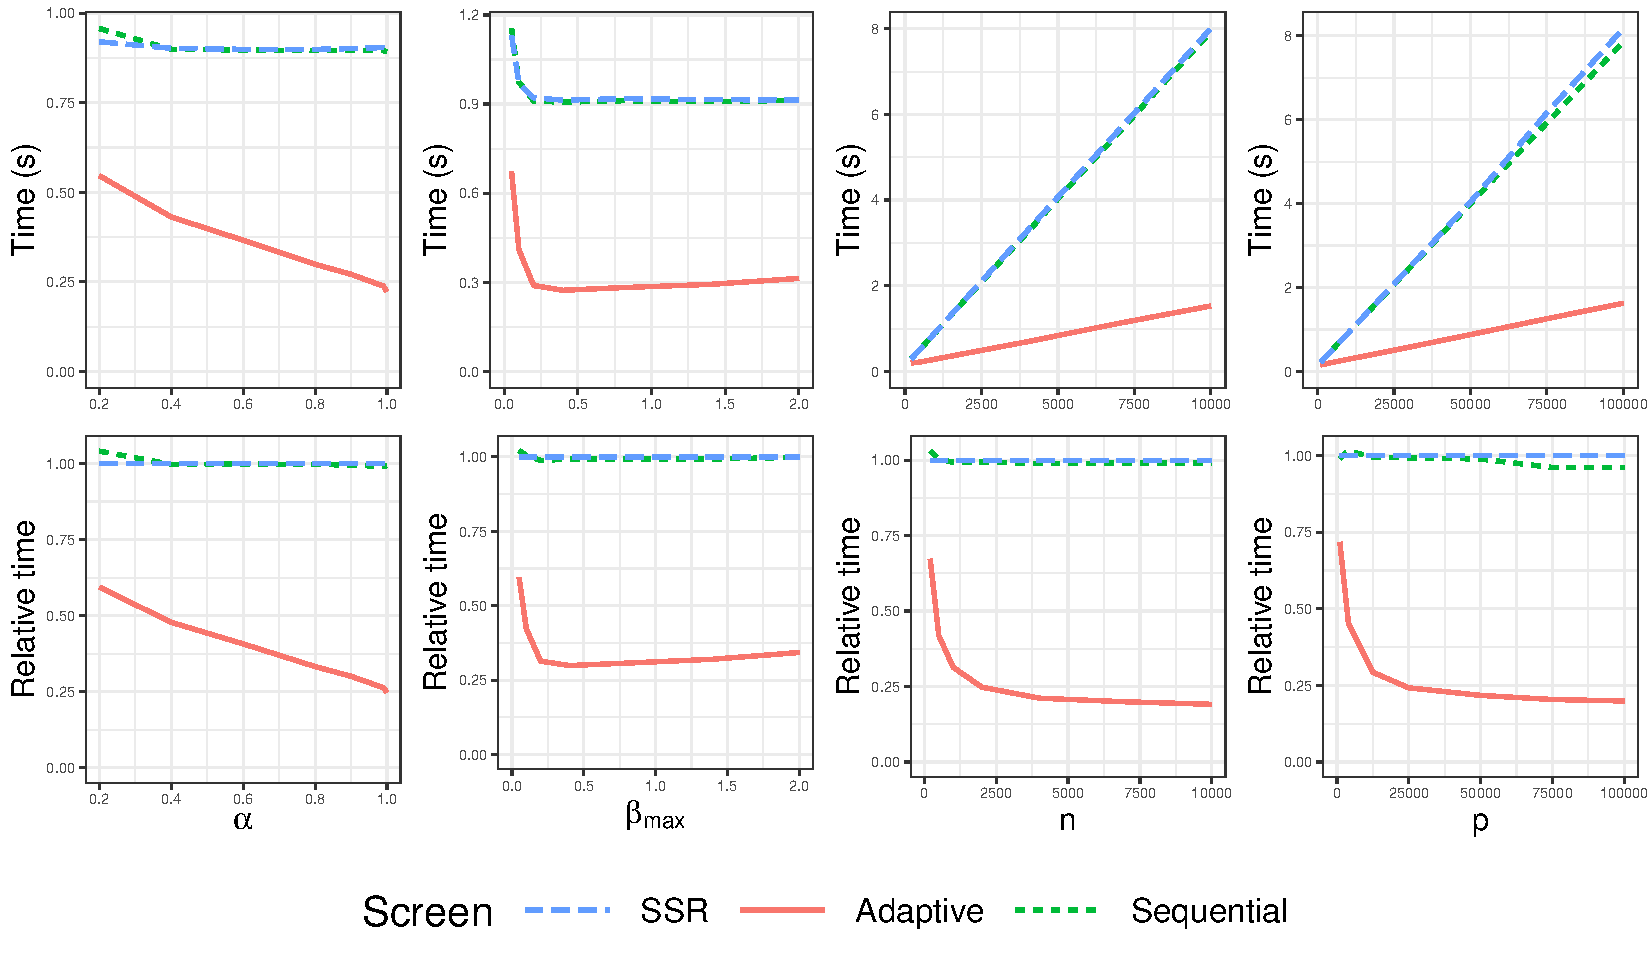
\includegraphics[width=\textwidth]{enet1.pdf}    \caption[Comparison of screening methods for elastic net in simulation 1]{Comparing speed of screening methods for elastic model under different settings. Top row: computation time in seconds. Bottom row: relative computation time compared to SSR. First column: Varying proportion of lasso penalty: $\alpha$. Second column: varying sample size $n$. Third column: varying number of features $p$. Fourth column: varying signal strength $\beta_{\max}$.}
    \label{fig:sim1}
\end{figure}

\begin{figure}[ht]
    \centering
    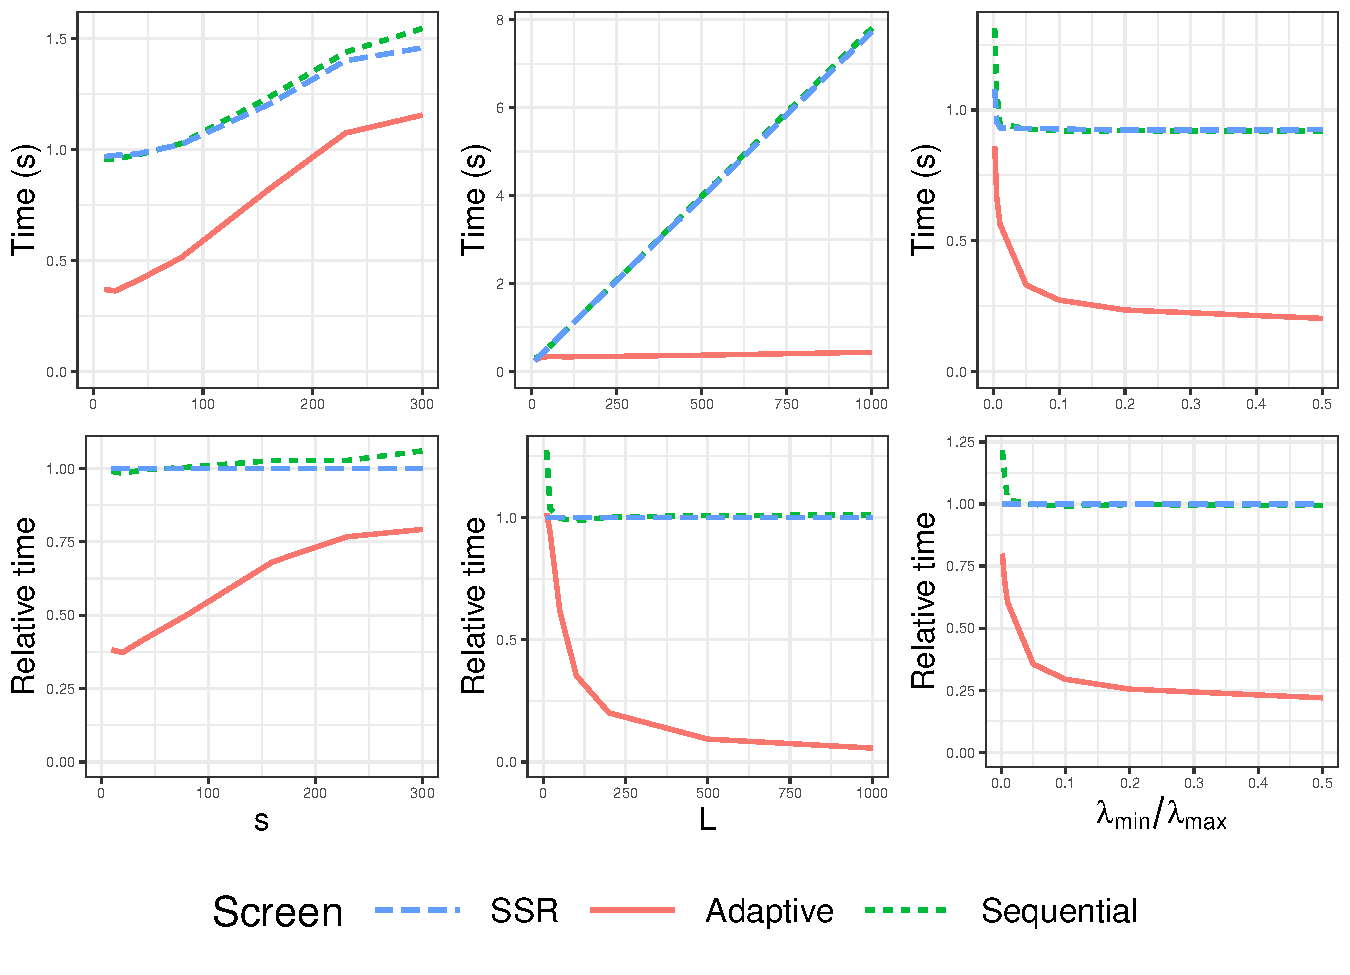
\includegraphics[width=0.82\textwidth]{enet2.pdf}    \caption[Comparison of screening methods for elastic net in simulation 2]{Comparing speed of screening methods for elastic net model under different settings. Top row: computation time in seconds. Bottom row: relative computation time compared to SSR. First column: varying sparsity $s$. Second column: Varying number of grid points $L$. Third column: Varying range of grid $\lambda_{\min}/\lambda_{\max}$.}
    \label{fig:sim2}
\end{figure}

The time spent on solving the whole path in seconds and the relative time compared to SSR method are summarized in Figures \ref{fig:sim1} and \ref{fig:sim2}, and form the basis for several observations. First, the sequential version of SPARSE rule performs almost the same as SSR except in some extreme cases, and the adaptive version of SPARSE rule outperforms the other two methods universally, with 3-4 $\times$ speedup in most cases. Second, the proposed adaptive method has the best performance when $\alpha$ is close to $1$, where the solutions are more sparse. Note that $\alpha=1$, which corresponds to the lasso problem, is included in the experiment, showing that our proposed method smoothly extends from the lasso problem to a larger class of elastic net problems. Third, adaptive screening is most favorable in high-dimensional settings with large $n$ and/or $p$, a small number of important features $s$, and for paths where $\lambda$ values are closely spaced, either because the number of points on the path $L$ is large or the path focuses on larger $\lambda$ values (larger $\lambda_{\min}/\lambda_{\max}$). Last, the effect of the signal strength $\boldsymbol\beta_{\max}$ has an interesting pattern. One would expect that as the signal becomes stronger, screening methods perform better at eliminating features, which is true in the first half of the range of $\boldsymbol\beta_{\max}$. After that, however, increasing $\boldsymbol\beta_{\max}$ seems to have a negative effect on the adaptive method. The reason may be that by introducing an extra variable $\boldsymbol\gamma$, the SPARSE rule becomes loose when $\boldsymbol\beta$ is large. Nevertheless, the adaptive method is still much faster than other methods regardless of the signal strength. We have also checked other factors, such as auto-correlation or block-correlation among the features and number of threads in parallel computing, but do not include these results as no interesting patterns were observed.

\subsection{Real Data}

\subsubsection{Traditional Data Sets}

In this section we compare the three screening methods on four real data sets with a variety of high-dimensional structures. An elastic net problem is solved along a grid of $L=100$ $\lambda$ values equally spaced on log scale between $(\lambda_{\max},\lambda_{\min}]$ where $\lambda_{\max}$ is determined by data and $\lambda_{\min}/\lambda_{\max}=0.05$. The 4 data sets are:

\begin{enumerate}
    \item \textbf{Breast cancer gene expression data
(GENE, \url{https://myweb.uiowa.edu/pbreheny/data/bcTCGA.html}):} this data has expression measurements of $p=17,322$ genes from $n=536$ patients. The response is the expression measurement of the gene BRCA1, which has been identified to be related to risk of breast cancer.
    \item \textbf{Cardiac fibrosis genome-wide association data
(GWAS, \url{https://arxiv.org/abs/1607.05636}):} this data set has $p=660,496$ single nucleotide
polymorphisms (SNPs) collected from $n=313$ human hearts. The response is the log of the ratio of cardiomyocytes to fibroblasts in the heart tissue, which is associated with heart failure.
    \item \textbf{MNIST handwritten image data
(MNIST, \url{http://yann.lecun.com/exdb/mnist}):} this data set has $60,000$ images in the training set and $10,000$ images in the testing set. Each image is a $28\times 28=784$ pixels image of handwritten digits. We use the training set to form a $n=784\times p=60,000$ feature matrix, treating pixels as samples and images as features. Then an image from the testing set is randomly selected as the response.
    \item \textbf{Subset of New York Times bag-of-words data
(NYT, \url{https://archive.ics.uci.edu/ml/datasets/Bag+of+Words}):} the raw data set is a $300,000\times 102,660$ matrix, each row being a document and each column being number of occurrence of a specific word in those documents. We selected $n=5,500$ documents by removing documents with low word counts. Then $55,000$ words are selected as the features and a randomly selected word is the response.
\end{enumerate}

For the GENE and GWAS data sets, the experiment is replicated 10 times, and the for the MNIST and NYT data sets, because the response is randomly selected, the experiment is replicated 50 times. Figure \ref{fig:real} summarizes the comparison of time spent on solving the whole path with different screening methods and $\alpha$ values on the 4 data sets. The proposed adaptive method is always fastest, especially when $\alpha$ is close to 1. However, the extent of the benefit varies considerably across the four data sets, which have very different correlation structures and signal strengths.

\begin{figure}[ht]
    \centering
    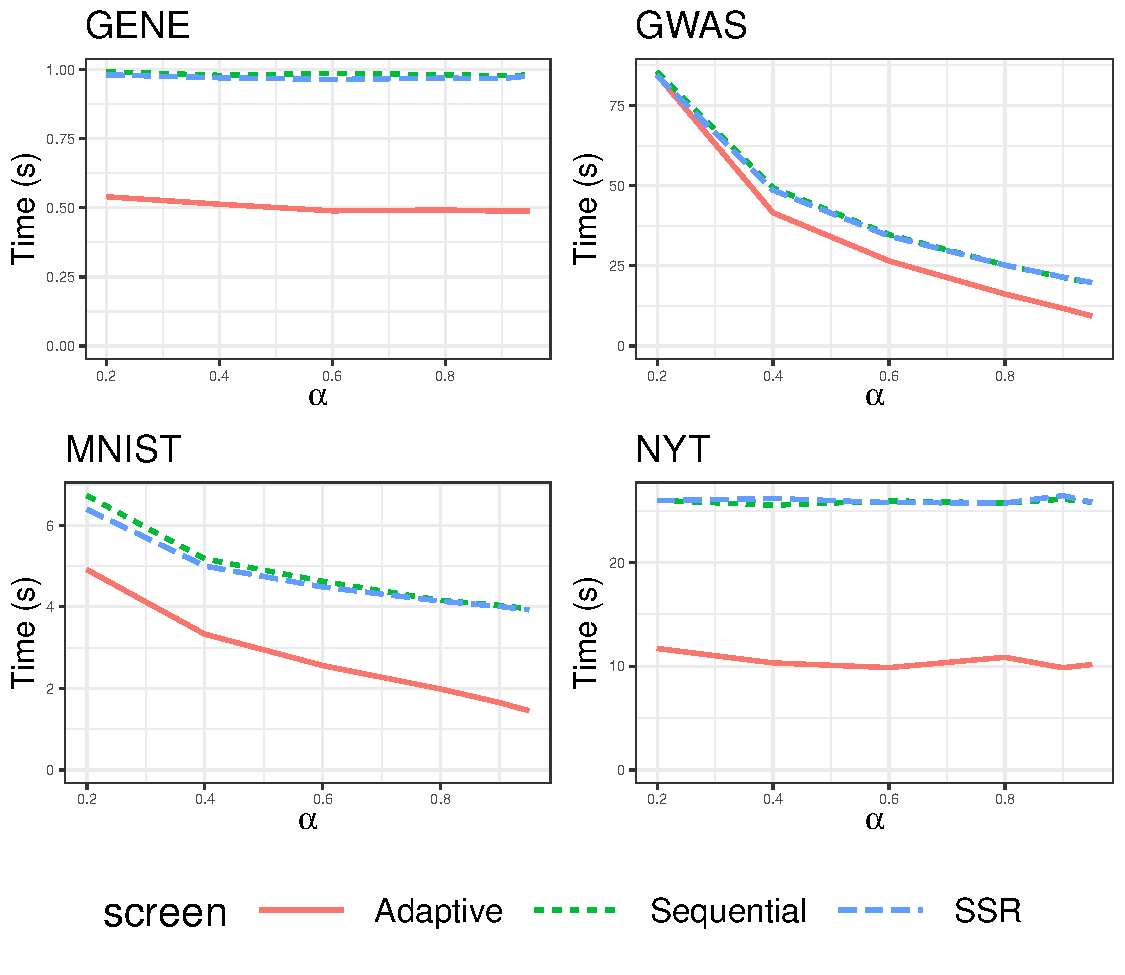
\includegraphics[width=0.82\textwidth]{enetreal.pdf}    \caption[Comparison of screening methods for elastic net on 4 data sets by $\alpha$]{Average computing time in seconds with different screening methods and $\alpha$ for elastic net model on 4 data sets.}
    \label{fig:real}
\end{figure}

\iffalse
\begin{table}[ht]
\centering
\begin{tabular}{llll}
\toprule
Screening method & SSR & Sequential & Adaptive  \\
\midrule
$\alpha=0.95$ & 945 (4) & 949 (3) & \textbf{455 (2)} \\
$\alpha=0.9$ & 946 (3) & 949 (4) & \textbf{465 (2)}  \\
$\alpha=0.8$ & 939 (2) & 948 (2) & \textbf{471 (2)}  \\
$\alpha=0.6$ & 936 (2) & 949 (2) & \textbf{485 (2)}  \\
$\alpha=0.4$ & 938 (1) & 949 (1) & \textbf{500 (1)}  \\
$\alpha=0.2$ & 953 (4) & 966 (2) & \textbf{544 (3)} \\
\bottomrule
\end{tabular}
\caption{Average computing time in millisecond (standard error) for the GENE data set}
\label{Tab:gene}
\end{table}
\fi

\subsubsection{Ultra High-dimensional Data Sets}

In this section, we consider an ultra high-dimensional real data set that cannot be fit into memory. This scenario presents the greatest challenge to optimization and is when a good screening method is most important. The Genetic Risk Assessment of Defibrillator Events study (GRADE, \url{https://www.clinicaltrials.gov/ct2/show/NCT02045043}) collected genome-wide data on 1,080 subjects diagnosed with cardiomyopathy and who had undergone surgery to receive an implantable cardioverter defibrillator in the past 5 years. After imputation using the Haplotype Reference Consortium as a reference genome and filtering for quality control \citep{Das2016}, there were $p=11,830,470$ SNPs which used as features. The size of the file storing the feature matrix is 96G and we conduct the test on a machine with 32G RAM. A variety of clinical data was collected on these individuals. To examine the performance of screening methods for elastic net problem, we focused on the numeric response left ventricular ejection fraction (LVEF). LVEF measures the proportion of blood being pumped out of the left ventricle of the heart with each contraction. Lower values are associated with more severe heart disease. LVEF data was available for $n=973$ subjects and they will be considered as the sample for this analysis. We chose a relatively large $\lambda_{\min} =0.1\lambda_{\max}$ to avoid having far more features selected than the number of observations. Even so, this choice led to solution paths with $1106$ to $4791$ features selected at the end of the path, depending on the value of $\alpha$. We choose number of $\lambda$ values to be the default value $L=100$ and test a grid of $\alpha$ values $\{1,0.95,0.9,0.8,0.6,0.4,0.2\}$. The time spent to solve the whole path in minutes for different screening methods and $\alpha$'s is shown in Figure~\ref{fig:lvef}. 

\begin{figure}[ht]
    \centering
    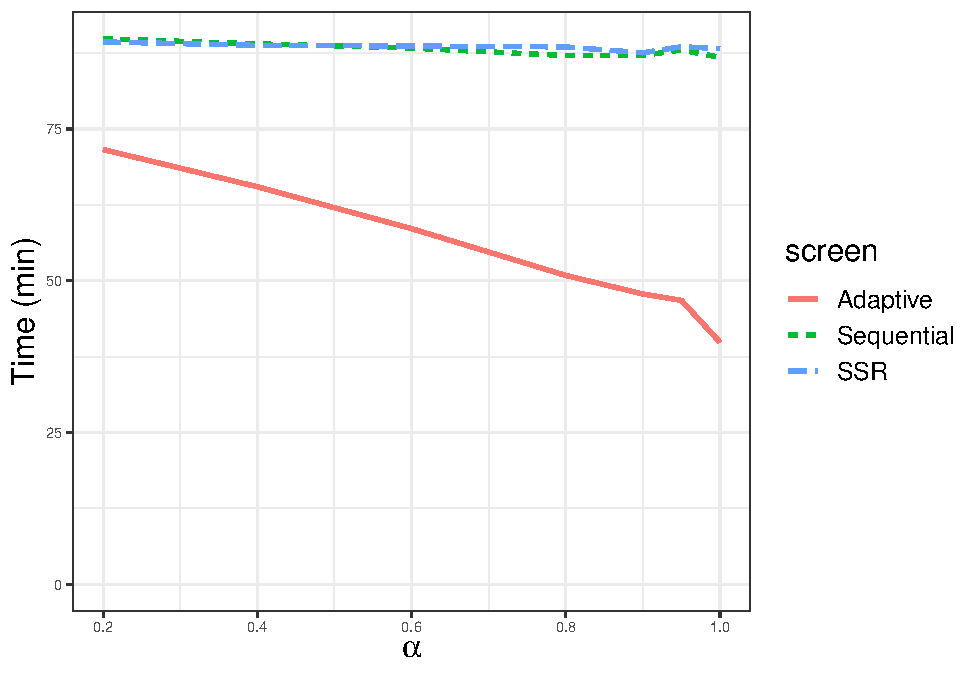
\includegraphics[width=0.72\textwidth]{enetlvef.pdf}    \caption[Comparison of screening methods for elastic net on LVEF analysis by $\alpha$]{Average computing time in minutes with different screening methods and $\alpha$ for elastic net model on GRADE data set.}
    \label{fig:lvef}
\end{figure}

\iffalse
\begin{table}[ht]
\centering
\begin{tabular}{llllll}
\toprule
Screening method & SSR\,\,\,\,\,\,\,\,\,    & Sequential   & Adaptive  \\
\midrule
$\alpha=1$ & 87.6 & 89.3 & \textbf{52.3}  \\
$\alpha=0.95$ & 87.5 & 89.6 & \textbf{61.5}  \\
$\alpha=0.9$ & 88.1 & 89.5 & \textbf{66.8}  \\
$\alpha=0.8$ & 87.6 & 89.7 & \textbf{72.2}  \\
$\alpha=0.6$ & 88.2 & 90.7 & \textbf{77.8} \\
$\alpha=0.4$ & 88.8 & 91.7 & \textbf{84.4}  \\
$\alpha=0.2$ & \textbf{89.3} & 94.5 & 91.1  \\

\bottomrule
\end{tabular}
\caption{Average computing time in minutes the LVEF analysis with elastic net.\label{Tab:lvef}}
\end{table}
\fi

The proposed adaptive screening is the fastest in most cases, especially in the case when $\alpha$ is large. Even if $\alpha$ is extremely small, it does not do much harm to the speed. The proposed sequential screening performs very similar to strong rule screening.



